%---------------------------------------------------------------------------------------

\chapter[Resultados]{Resultados}\label{ch:resultados}

%---------------------------------------------------------------------------------------

% Lista de abreviaturas e de siglas

%---------------------------------------------------------------------------------------

% Lista de simbolos

%---------------------------------------------------------------------------------------

\section{Validação: tubo de choque de Sod}\label{sec:validacao:-tubo-de-choque-de-sod}

A validação numérica foi realizada com o problema clássico do tubo de choque de Sod em 1D, com condições iniciais descontínuas:

\[
(\rho,u,p)=
\begin{cases}
(\rho_L,0,p_L), & x < x_0,\\
(\rho_R,0,p_R), & x \ge x_0,
\end{cases}
\qquad \text{com } \rho_L>\rho_R,\ p_L>p_R.
\]

As grandezas de interesse são os perfis de densidade, velocidade e pressão no tempo adimensional \(t^\ast\).
Para avaliar a acurácia, foi executada uma análise de convergência variando o número de lattices \(N_x\) ao longo da direção longitudinal do domínio, mantendo as propriedades do escoamento constantes.

O erro quadrático médio (EQM) foi computado para a pressão,
\[
\mathrm{EQM}(p)=\left( \frac{1}{N_x}\sum_{i=1}^{N_x}\big(p_i - p_i^{\mathrm{ref}}\big)^2 \right)^{1/2},
\]
e analogamente para \(\rho\) e \(u\).
A solução de referência \(p^{\mathrm{ref}}\) foi obtida pela solução analítica do problema de Riemann de Sod (método exato de duas ondas) amostrada nos mesmos pontos \(x_i\) e mesmos tempos \(t_j\).

A Figura~\ref{fig:convergence} apresenta a variação do EQM em função de \(N_x\) em escala log–log.
Observa-se regime aproximadamente de primeira ordem, consistente com a presença de descontinuidades dominando a norma do erro.
O aumento da razão de pressões \(\Pi\) degrada a acurária dos resultados, sendo obtido uma razão máxima de \(\Pi=20\) antes de ocorrer divergência numérica irreversível na simulação.
Para \(\rho\) e \(u\), o comportamento é análogo, com leve superconvergência em regiões suaves.

\begin{figure}[h!]
  \centering
  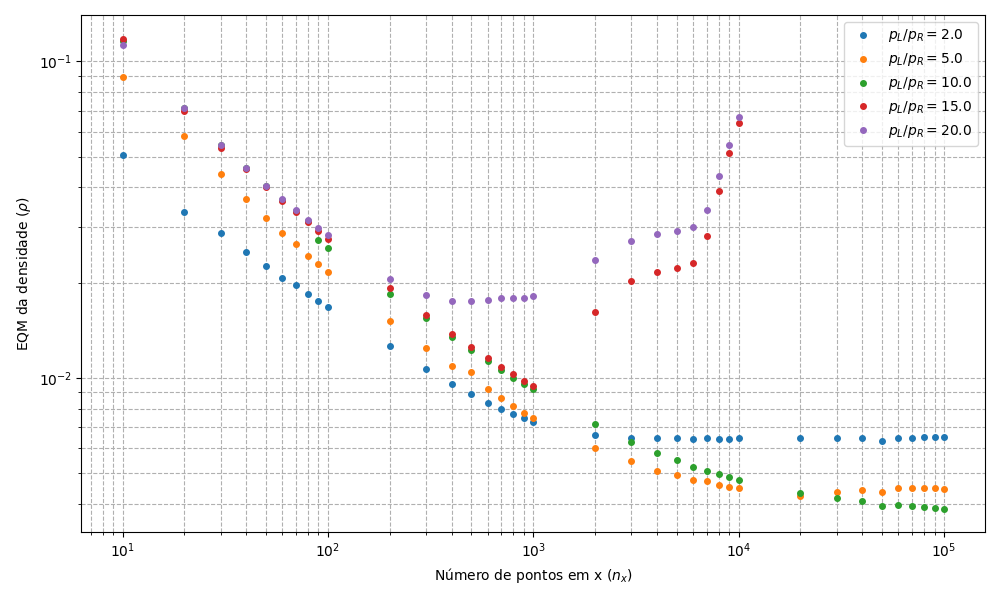
\includegraphics[width=0.8\linewidth]{fig/convergence.png}
  \caption{Convergência no tubo de choque de Sod: EQM em função do número de lattices \(N_x\) e razão de pressões \(\Pi=p_L^\star/p_R^\star\) comparada à solução de referência.}
  \label{fig:convergence}
\end{figure}

\section{Escalabilidade em CPU multinúcleo}\label{sec:escalabilidade-em-cpu-multinucleo}

A escalabilidade foi avaliada em um processador Intel Core 7--240H com seis núcleos de performance, utilizando 1 a 6 núcleos para malhas 1D com \(N_x=10^3\) e \(N_x=10^4\).
Mantivemos o mesmo número de passos de tempo e configuração física para isolar efeitos de paralelização.
O tempo de execução \(T(p)\) foi normalizado pelo caso sequencial \(T(1)\).
As métricas são:
\[
S(p)=\frac{T(1)}{T(p)},\qquad
E(p)=\frac{S(p)}{p}.
\]

A Figura~\ref{fig:scalability} mostra o fator de aceleração \(S(p)\) para \(p=1,\dots,6\) a partir da média aritmética de três medidas para cada caso.
Para \(N_x=10^3\), observamos escalabilidade quase linear, com eficiência acima de 80\% em todos os testes.
Para \(N_x=10^4\), a sobrecarga de paralelização torna-se mais relevante, reduzindo \(E(p)\) especialmente acima de 5 núcleos, coerente com a pressão de memória e sincronizações de borda.
O perfil indica que o kernel de colisão–streaming é bound por largura de banda de memória em regimes mais finos, enquanto o custo de comunicação (bordas/partições) limita ganhos para problemas menores.

\begin{figure}[h!]
  \centering
  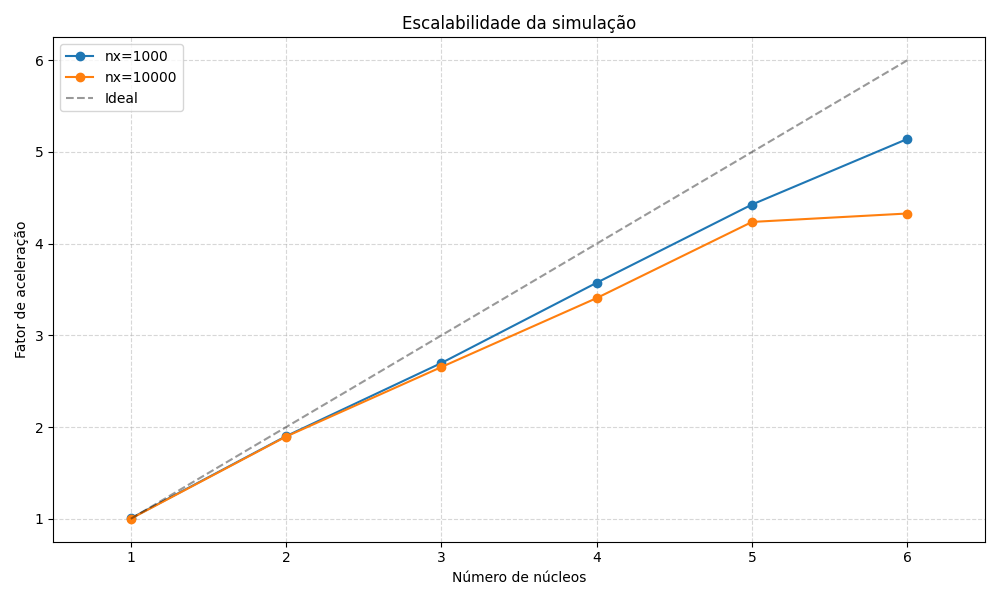
\includegraphics[width=0.8\linewidth]{fig/scalability.png}
  \caption{Escalabilidade em CPU: aceleração \(S(p)\) para 1–6 núcleos no Intel Core 7--240H, com \(N_x=10^3\) e \(N_x=10^4\).}
  \label{fig:scalability}
\end{figure}
